\documentclass[12pt, letterpaper]{article}
\usepackage{graphicx}
\usepackage{scicite}

\usepackage{times}

\usepackage{graphicx}
\graphicspath{{./Figures/}}
\usepackage{amssymb}
\usepackage{amsmath}
\usepackage{wasysym}
\usepackage{caption}


\title{Tidal Evolution of the Earth-Moon System}
\author{Rishik Adhikari (Student Number: 1008214905) }
\date{May 15 2023}

\begin{document}

\maketitle

\section*{Introduction}

In This Project, Tidal Evolution of Earth and Moon is examined. In our everyday life, we can see or experience tidal effects near beaches of seas and oceans. Moon's gravity is one of the main cause of these tidal effects on Earth. By Studying The tidal evolution of Earth and Moon, we can learn many more information about these bodies. Such as age estimation, length of day estimations over time, and many more. The goal of this project is to answer some of the questions using a tidal evolution model guided by the following equations:

    \begin{eqnarray}
        \frac{dL_\oplus}{dt} &=& T_\odot,\\
        \frac{dS_\oplus}{dt} &=& -T_\odot-T_{\leftmoon},\\
        \frac{dL_{\leftmoon}}{dt} &=& T_{\leftmoon}.
    \end{eqnarray}

We will solve this differential Equations using odeint function from scipy library in Python Programming Language. Initial Conditions Required to solve the ode is as follow:

\begin{eqnarray}
L_\oplus &=& M_\oplus\sqrt{G(M_\odot + M_\oplus) a_\oplus},\\
S_\oplus &=& I\Omega_\oplus,\\
L_{\leftmoon} &=& m_{\leftmoon}\sqrt{G(M_\oplus+m_{\leftmoon}) a_{\leftmoon}}.
\end{eqnarray}.

Some Other Important Relations and Equations Required to solve the ode. They are as follow:

\begin{eqnarray}
  T_{\leftmoon} &=& \frac{3}{2}\frac{G m^2_{\leftmoon}}{a_{\leftmoon}}\left(\frac{R_\oplus}{a_{\leftmoon}}\right)^5 \frac{k_2}{Q_{\leftmoon}}. \\
  T_{\odot} &=& T_{\leftmoon}*\frac{1}{4.7}
\end{eqnarray}

\section*{Solution Approach}

Please Refer to the Github Ipynb file for all the Code used in this Project. I will briefly explain what I did in Points.

\begin{itemize}
  \item I picked CGS system of Unit to solve almost all the problems in this Project.
  \item In Question 5. The Given ODE is solved using scipy.integrate.odeint in Python Programming.
  \item I integrated approximately upto 5 billion years ago using seconds as the unit of time. 
  \item t = [0,-1.5e17] is the time-interval used in odeint. 1.5e17 in seconds is approximately equal to 5 billion years.
  \item Spin Angular Momentum of Earth Calculated by solving the ODEs is used to find length\_of\_day(t) for Question 7. 
  \item Equation 6, along with Orbital Angular Momentum of Moon, Computed By solving the ODEs is used to solve for the $a_{\leftmoon}$ (t) for Question 6.  
  \item Moon Formation Happened Approximately 1.6 Billion Years Ago According to the Model, which is very off from the actual value of 4.7 Billion Years.
  
\end{itemize}

\section*{Question 9}

\textbf{Age of Moon:} About 4.47 billion years old. Compared to The Tidal Model used in this Assignment, the Prediction by The Tidal Model is way off by almost 2.8 billion years.\\ \\
\textbf{Age of Earth:} About 4.54 billion years old, plus or minus about 50 million years.\\

\textbf{Source Links:}
\begin{itemize}
    \item https://education.nationalgeographic.org/resource/resource-library-age-earth/
    \item https://www.nationalgeographic.com/science/article/140402-moon-formation-earth-age-space-science \\ \\
\end{itemize}

\section*{Question 10}

\textbf{Estimation: } Estimation of the Age of Earth and Moon using the Tidal Model in the Assignment, is very off from the actual age. \\ \\
\textbf{The Possible Problems Could be the computation limit and the dependence of all the Differential Equations to the semi-major axis of the Moon. } 
\begin{itemize}
    \item Even though arithmetic calculation using a computer seems very fast and accurate, it has limitation when it comes to computation, Especially with floating Point. So Probably, the orbital angular momentum as they approach zero are treated as actual zero, which affected the age Estimation of Earth and Moon.
    \item Also, derivative of orbital angular momentum and the spin angular momentum of Earth, depend on the semi-major axis of the Moon. So, as soon as the semi-major axis of Moon goes to zero, any further data of Earth Collected using this model, becomes invalid too.\\ \\
\end{itemize}
\newpage

\textbf{Some Useful Figures Plotted in the Project Ipynb Document Are Displayed Below:}

\begin{figure}[!htb]
    \centering
    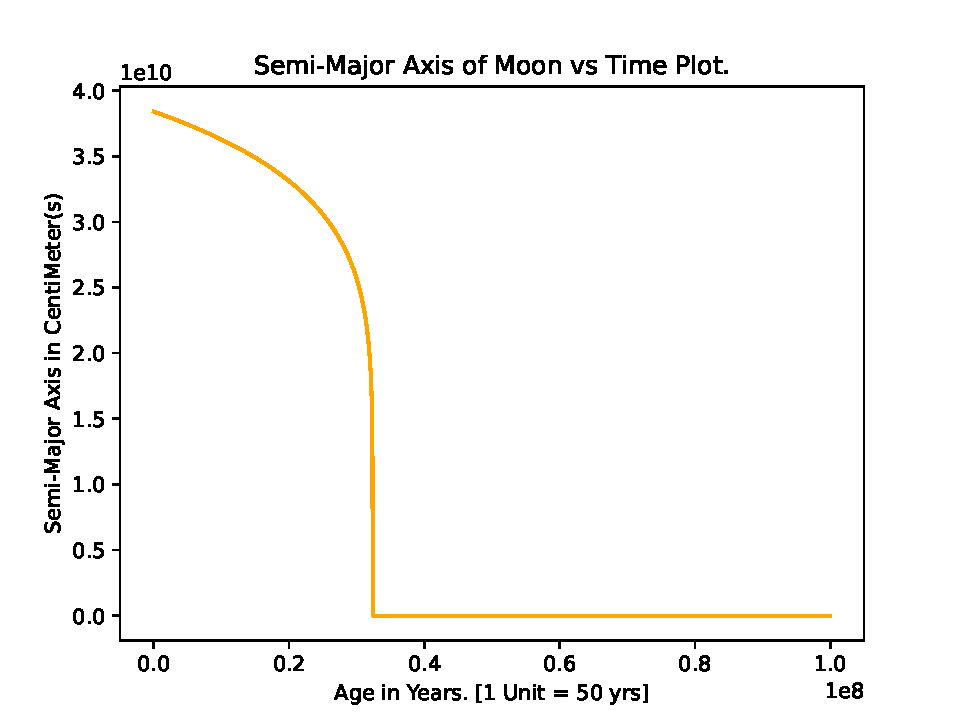
\includegraphics[scale=0.9]{Q6.pdf}
    \caption{Plot of Question 6. Age/Time Vs Semi-Major Axis of Moon.}
    \label{fig:Q6.pdf}
\end{figure}
\begin{figure}[!htb]
    \centering
    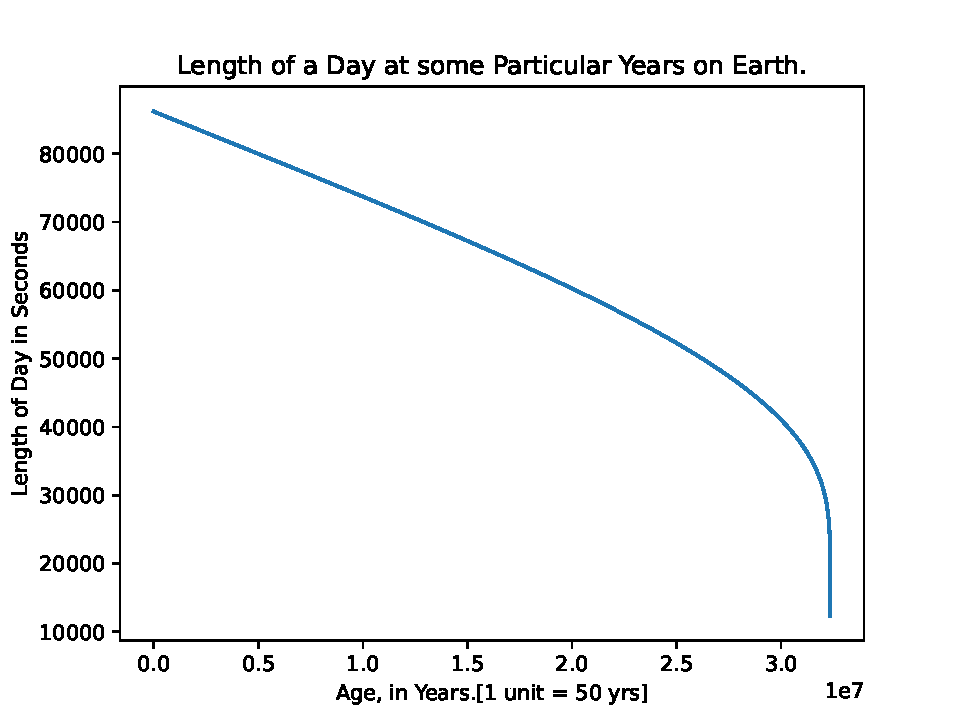
\includegraphics[scale=0.9]{Q72.pdf}
    \caption{Plot of Question 7. Age/Time Vs Semi-Major Axis of Moon.}
    \label{fig:Q72.pdf}
\end{figure}

\newpage
\section*{Conclusion}

In Conclusion, The Tidal Evolution Model of Earth-Moon used in This Project is not very efficient and the estimation of the age of Moon was very off from the actual value. However, it is a very good project for students to learn various computational techniques including but not limited to solving numerical integrations, plotting, writing report in Latex, etc. 

\end{document}
